\section{Ziel}
In diesem Versuch wird das Verhalten von parallel und senkrecht polarisiertem Licht bei Reflexion an Grenzflächen untersucht,
d.h. es werden die Fresnelschen Gleichungen für die Reflexion überprüft.
Außerdem wird der Brewsterwinkel sowie der Brechungsindex von Silizium ermittelt.


\section[Theorie]{Theorie\footnote[1]{Unter Verwendung von \cite{man:v407}.}}

\subsection{Polarisation}
Elektromagnetische Wellen schwingen stets senkrecht zu ihrer Ausbreitungsrichtung.
Je nach der Form, mit der sich das elektrische bzw. magnetische Feld dabei bewegt,
wird beispielsweise von linear polarisiertem Licht (die Felder schwingen auf einer Geraden senkrecht zur Ausbreitung)
oder zirkular polarisiertem Licht (die Felder schwingen auf einem Kreis senkrecht zur Ausbreitung) gesprochen.
In diesem Versuch ist das linear polarisierte Licht von Interesse, das beispielsweies mittels Polarisationsfolien aus unpolarisiertem Licht erzeugt werden kann.
Trifft Licht auf eine Grenzfläche, wird es zum Teil transmittiert und zum Teil reflektiert.
Die Einfallsebene ist dann die Ebene, die vom einfallenden, transmittierten und reflektierten Lichtstrahl aufgespannt wird, vgl. Abbildung \ref{fig:einfallsebene}.
Linear polarisiertes Licht, das parallel bzw. senkrecht zur Einfallsebene schwingt, wird parallel bzw. senkrecht polarisiert genannt.


\begin{figure}[H]
    \centering
    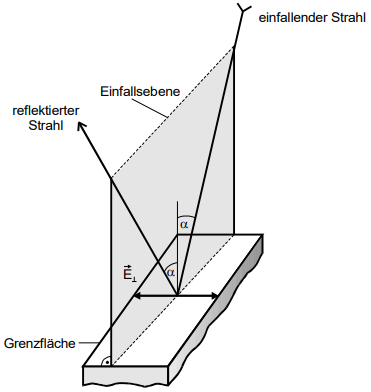
\includegraphics[height = 6 cm]{Abbildungen/einfallsebene.png}
    \caption{Darstellung der Einfallsebene bei der Reflexion an einer ebenen Grenzfläche \cite{man:v407}.}
    \label{fig:einfallsebene}
\end{figure}

\subsection{Die Fresnelschen Gleichungen}
% Trifft Licht auf eine Grenzfläche zwischen zwei Brechungsindizes, wird es zum Teil transmittiert und zum Teil reflektiert.
% Dabei ist unter anderem der Einfallswinkel ausschlaggebend.
Theoretische Grundlage dieses Versuchs sind die Maxwellschen Gleichungen
\begin{align}
    \nabla \times \symbf{H} &= \symbf{j} + \epsilon \epsilon_0 \dot{\symbf{E}}
     & \nabla \times \symbf{E} &= - \mu \mu_0 \dot{\symbf{H}}
\end{align}
mit der Dielektrizitätskonstante $\epsilon$ und der elekrischen Feldkonstante $\epsilon_0$ sowie der magnetischen Permeabilität $\mu$ und der Induktionskonstante $\mu_0$.
Dabei ist $\symbf{E}$ die elektrische Feldstärke und $\symbf{H}$ die magnetische Erregung.
Ferner gibt $\symbf{j}$ die elektrische Stromdichte an.
Im Folgenden werden nur nicht-ferromagnetische und nicht elektrisch leitende Materialien ($\mu = 1, \symbf{j} = 0$) betrachtet.
Aus den Maxwellschen Gleichungen lassen sich bestimmte Bedingungen für Licht als elektromagnetische Welle herleiten:

\noindent
Zum einen kann hergeleitet werden, dass Strahlung ein Energietransport ist, der durch den Poynting-Vektor
\begin{align}
    \symbf{S} = \symbf{E} \times \symbf{H},
    \label{eq:poynting}
\end{align}
beschrieben wird und für den kein Medium notwendig ist.
Die Strahlungsleistung pro Fläche beträgt
\begin{align}
    \left|\symbf{S}\right| = v \epsilon \epsilon_0 \symbf{E}^2
    \label{eq:leistung}
\end{align}
mit der Ausbreitungsgeschwindigkeit $v$ der Welle.

\noindent
Zum anderen kann unter Verwendung des Snelliusschen Brechungsgesetzes
\begin{align}
    \frac{n_2}{n_1} = \frac{\sin(\alpha)}{\sin(\beta)}
    \label{eq:snellius}
\end{align}
das Verhalten von elektromagnetischen Wellen an Grenzflächen zweier Materialien mit unterschiedlichen Brechungsindizes untersucht werden.
Dabei steht $n$ für den Brechungsindex des jeweiligen Mediums, $\alpha$ ist der Einfalls- und Reflexionswinkel und $\beta$ ist der Transmissionswinkel.
Der Brechungsindex $n$ beschreibt dabei das Geschwindingkeitsverhältnis der Welle im Vakuum im Vergleich zum betrachteten Material, also $n = c/v$.
Aus den Maxwellschen Gleichungen lässt sich ferner die Relation $n^2 = \epsilon$ herleiten.
Mit Hilfe dieser Relationen können schließlich die Fresnelschen Gleichungen für senkrecht und parallel polarisiertes Licht hergeleitet werden.
Für die Reflexion gilt bei senkrecht polarisiertem Licht
\begin{align}
    \symbf{E}_{\text{r}\perp} = - \symbf{E}_{\text{e}\perp} \frac{\left(\sqrt{n^2 -\sin^2\alpha} - \cos{\alpha}\right)^2}{n^2 - 1}
    \label{eq:senkrecht}
\end{align}
und bei parallel polarisiertem Licht
\begin{align}
    \symbf{E}_{\text{r}\parallel} = \symbf{E}_{\text{e}\parallel} \frac{n^2 \cos\alpha - \sqrt{n^2 - \sin^2\alpha}}{n^2 \cos\alpha + \sqrt{n^2 - \sin^2\alpha}}.
    \label{eq:parallel}
\end{align}
Dabei steht \enquote{e} für das einfallende und \enquote{r} für das reflektierte Licht.

\noindent
Gleichung \eqref{eq:parallel} kann wie folgt nach $n$ umgstellt werden:
\begin{gather}
    \nonumber E_{\text{r}\parallel} \left(n^2 \cos\alpha + \sqrt{n^2 - \sin^2\alpha}\right) 
    = E_{\text{e}\parallel} \left(n^2 \cos\alpha - \sqrt{n^2 - \sin^2\alpha}\right) \\
%
    \nonumber \iff \cos^2\alpha \left(E_{\text{r}\parallel} - E_{\text{e}\parallel}\right)^2 n^4 
    = \left(n^2 - \sin^2\alpha\right) \left(E_{\text{r}\parallel} + E_{\text{e}\parallel}\right)^2 \\
%
    \nonumber \iff \cos^2\alpha \left(E_{\text{r}\parallel} - E_{\text{e}\parallel}\right)^2 n^4
    - \left(E_{\text{r}\parallel} + E_{\text{e}\parallel}\right)^2 n^2 
    + \sin^2\alpha \left(E_{\text{r}\parallel} + E_{\text{e}\parallel}\right)^2  = 0\\ 
%
    \nonumber \iff n^4 - \frac{1}{\cos^2\alpha} \left(\frac{E_{\text{r}\parallel} + E_{\text{e}\parallel}}
    {E_{\text{r}\parallel} - E_{\text{e}\parallel}}\right)^2 n^2
    + \tan^2\alpha \left(\frac{E_{\text{r}\parallel} + E_{\text{e}\parallel}}
    {E_{\text{r}\parallel} - E_{\text{e}\parallel}}\right)^2 = 0\\
%
    \nonumber \iff n^2 = \frac{1}{2} \left(\frac{1}{\cos\alpha} 
    \frac{E_{\text{r}\parallel} + E_{\text{e}\parallel}}{E_{\text{r}\parallel} - E_{\text{e}\parallel}}\right)^2
    \pm \sqrt{\frac{1}{4} \left(\frac{1}{\cos\alpha} \cdot
    \frac{E_{\text{r}\parallel} + E_{\text{e}\parallel}}{E_{\text{r}\parallel} - E_{\text{e}\parallel}}\right)^4
    - \left(\tan\alpha \cdot \frac{E_{\text{r}\parallel} + E_{\text{e}\parallel}}
    {E_{\text{r}\parallel} - E_{\text{e}\parallel}}\right)^2}
\end{gather} 
Da $n > 0$ gelten muss, egibt sich schließlich
\begin{align}
    n = \sqrt{\frac{1}{2} \left(\frac{1}{\cos\alpha} 
    \frac{E_{\text{r}\parallel} + E_{\text{e}\parallel}}{E_{\text{r}\parallel} - E_{\text{e}\parallel}}\right)^2
    \pm \sqrt{\frac{1}{4} \left(\frac{1}{\cos\alpha} \cdot
    \frac{E_{\text{r}\parallel} + E_{\text{e}\parallel}}{E_{\text{r}\parallel} - E_{\text{e}\parallel}}\right)^4
    - \left(\tan\alpha \cdot \frac{E_{\text{r}\parallel} + E_{\text{e}\parallel}}
    {E_{\text{r}\parallel} - E_{\text{e}\parallel}}\right)^2}}.
    \label{eq:n_parallel}
\end{align}
Auf ähnliche Art und Weise lässt sich Gleichung \eqref{eq:senkrecht} ebenfalls nach $n$ umstellen.
Da die Rechnung hier allerdings deutlich komplizierter verläuft, wird die Herleitung mittels des Online-Tools WolframAlpha \cite{wolfram_n}
durchgeführt.
Es ergibt sich in diesem Fall
\begin{align}
    n = \frac{\sqrt{E_{\text{r}\perp}^2 + E_{\text{e}\perp}^2 - 2 E_{\text{r}\perp} E_{\text{e}\perp} \cos(2\alpha)}}
    {E_{\text{r}\perp} + E_{\text{e}\perp}}.
    \label{eq:n_senkrecht}
\end{align}

\subsection{Brewsterwinkel}
Bei externer Reflexion (optisch dünn auf dicht) gibt es einen gewissen Winkel, den sogenannten Brewsterwinkel, bei dem kein 
parallel polarisiertes Licht reflektiert wird.
Mathematisch bedeutet dass, dass $\symbf{E}_{\text{r}\parallel}$ in Gleichung \eqref{eq:parallel} einen Nulldurchgang hat.
Die Bedingung hierfür lautet $\alpha_\text{B} + \beta_\text{B} = \qty{90}{\degree}$.
Nach Snellius \eqref{eq:snellius} folgt dann für $n_1 = n_\text{Luft} = 1$ und $n_2 = n$
\begin{align}
    \alpha_\text{B} = \arctan n.
    \label{eq:brewster}
\end{align}

%Brewsterwinkel
